\documentclass[11pt]{article}

\usepackage{a4wide}
\usepackage{graphicx}
\bibliographystyle{plain}

\begin{document}

\section{Introduction}

This is a sample file. The quick brown fox jumped over the lazy cow at
same time that it was time for all good people to come to the aid of
the party. The quick brown fox jumped over the lazy cow at
same time that it was time for all good people to come to the aid of
the party. The quick brown fox jumped over the lazy cow at
same time that it was time for all good people to come to the aid of
the party.

\begin{center}
\begin{tabular}{lr}
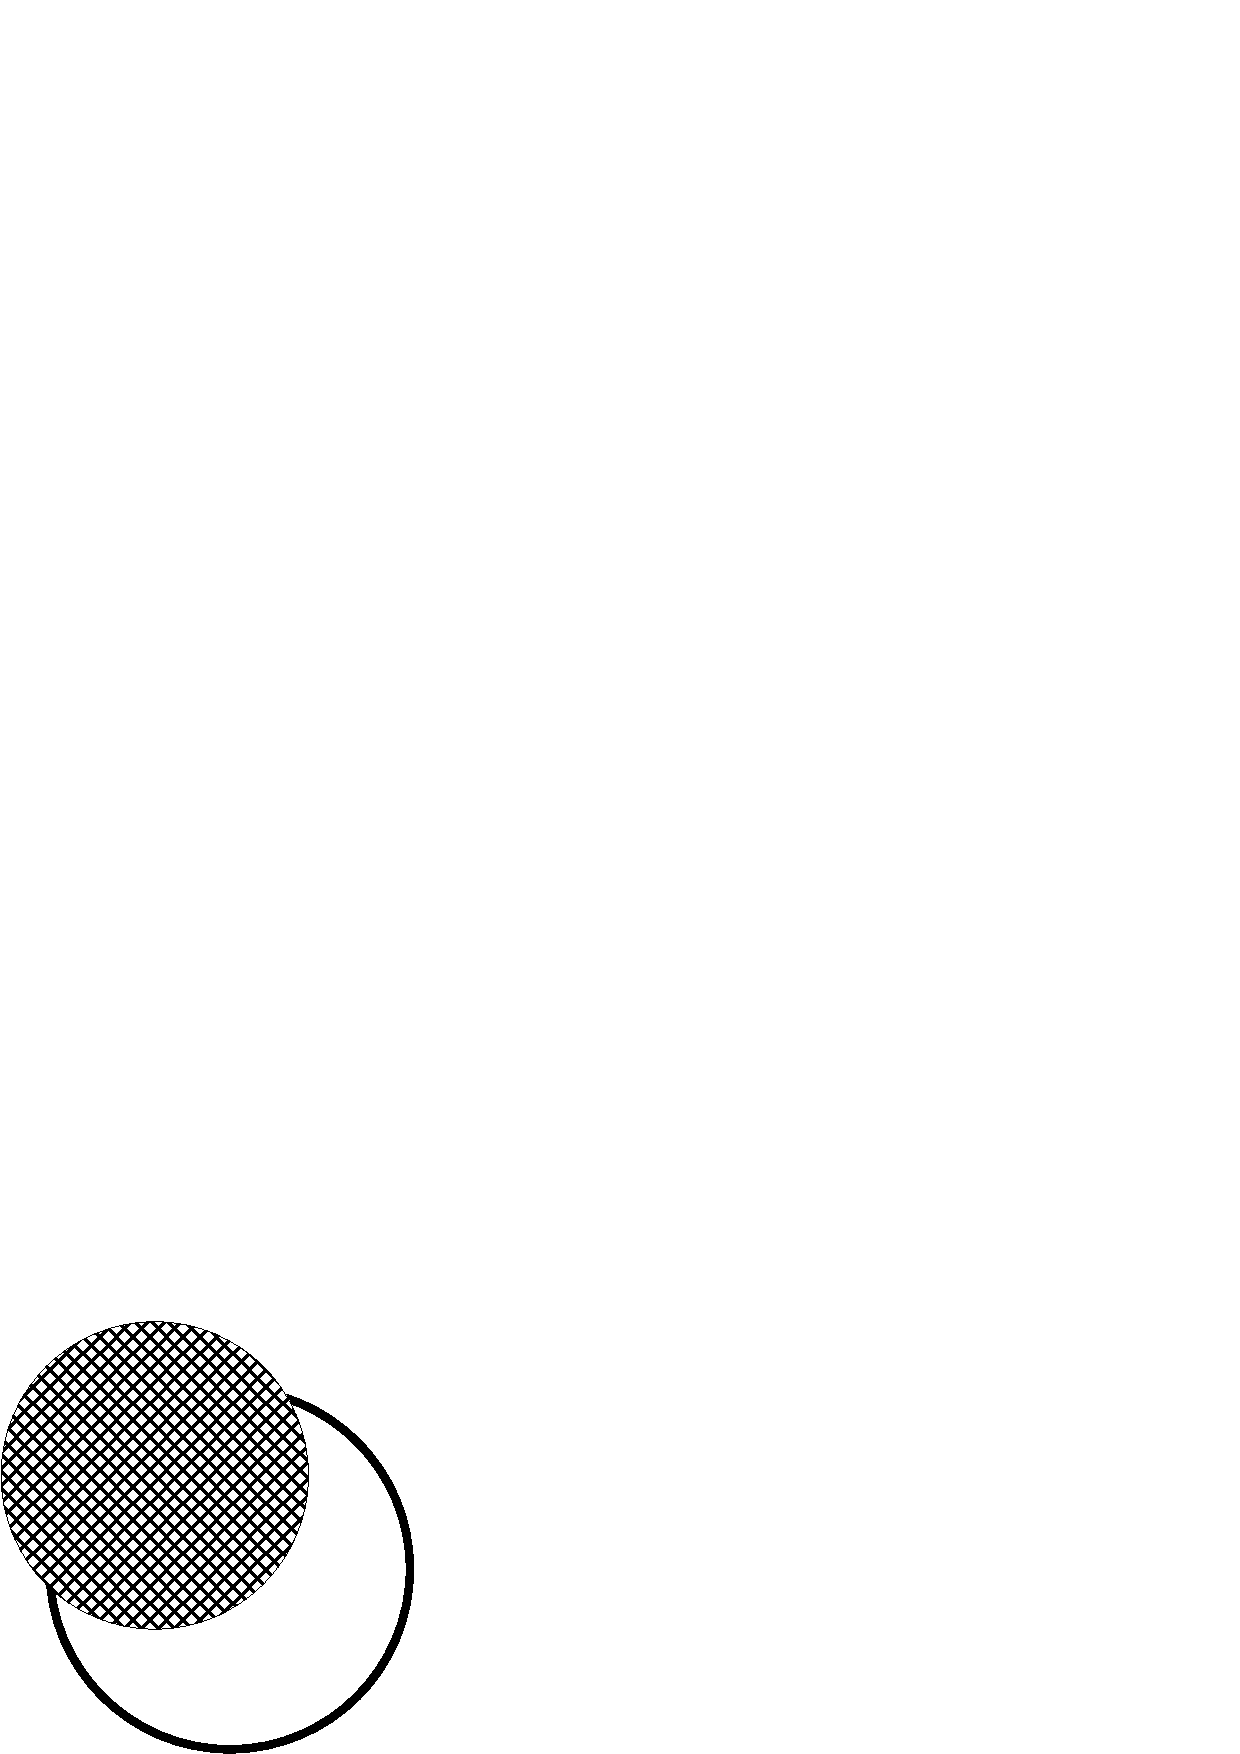
\includegraphics[scale=0.4]{circle.pdf}
& 
\includegraphics[scale=0.4]{square.pdf}
\end{tabular}
\end{center}

\noindent
We can prove that this is not an optimal way of representing data. For
example, suffix arrays \cite{manber93} are a well known approach.

\section{Some more things}

This is a sample file. The quick brown fox jumped over the lazy cow at
same time that it was time for all good people to come to the aid of
the party. The quick brown fox jumped over the lazy cow at
same time that it was time for all good people to come to the aid of
the party. The quick brown fox jumped over the lazy cow at
same time that it was time for all good people to come to the aid of
the party.

\section{Reference}

\bibliography{refs}

\end{document}

%%% Local Variables: 
%%% mode: latex
%%% TeX-master: t
%%% End: 
